\documentclass[120.214pt]{article}%шаблон для статьи, шрифт 12 пт
\usepackage[utf8x]{inputenc} %использование кодировки Юникод UTF-8
\usepackage[russian]{babel} %пакет поддержки русского языка
\usepackage[compact]{titlesec}
\titlespacing*{\section}{0.75cm}{1em}{0.1em}
%\titlespacing{\заголовок}{слева}{перед}{после}[справа]

\usepackage{indentfirst}
\setlength{\parindent}{0.75cm}

\usepackage{amsmath}
\usepackage{amssymb}
\usepackage{graphicx}
\usepackage[labelsep=endash]{caption}
\usepackage{subcaption}
\usepackage{listings}

%\pagenumbering{gobble} % отключение нумерации страниц
\usepackage{fancyhdr}% загрузим пакет 
\pagestyle{fancy} %применим колонтитул
\fancyhead{}% очистим хидер на всякий случай
\fancyhead[R]{\thepage}% с какой стороны будет нумерация
\fancyfoot[C]{Учебник для чайников}
\setlength{\parindent}{0.75cm}




\begin{document} %начало документа
\section{Математика для чайников}
Что значит $ 4x^{2} + 5x -2$?
Для того, чтобы разобраться, вспомним, что такое Дискриминат.

Дискриминант --- это число, которое вычисляется так:
\begin{equation}
D = b^{2} - 4ac
\label{eq1}
\end{equation}

Несложно, верно?

Для вычисления $ x $ необходимо выполнить следующее:
\begin{equation}
\left\lbrace 
\begin{aligned}
x_{1} = \dfrac{-b - \sqrt{D}}{2a}\\
x_{2} = \dfrac{-b + \sqrt{D}}{2a}
\end{aligned}
\right.
\label{eq2}
\end{equation}

Иногда это записывают проще:
\begin{equation}
x_{1,2} = \dfrac{-b ± \sqrt{D}}{2a}
\label{eq3}
\end{equation}

Для (\ref{eq1}) необходимо помнить, что $ D \ge 0 $.
$ D \ne \phi $, $ \phi \in (-\infty ;0) $. Иначе невозможно будет вычислить (\ref{eq2}), (\ref{eq3}) в $ \mathbb{R} $.

\[ P^{rs} = P^{rs}_1 \cup P^{rs}_2, \forall rs \in RS \]

\section{Тригонометрия}
Наиболее часто встречающиеся значения синуса и косинуса приведены в таблице \ref{tab_sincos}.

\begin{table}[hb]
	\centering
	\caption{Значения синуса и косинуса}
	\label{tab_sincos}
\begin{tabular}{|c|c|c|c|c|}
	\hline 
	$ x $ & $ \dfrac{\pi}{6} $ & $ \dfrac{\pi}{4} $ & $ \dfrac{\pi}{3} $ & $ \dfrac{\pi}{2} $ \\ 
	\hline 
	$ sin $ & $ \dfrac{1}{2} $ & $ \dfrac{\sqrt{2}}{2} $ & $ \dfrac{\sqrt{3}}{2} $ & $ 1 $ \\ 
	\hline 
	$ cos $ & $ \dfrac{\sqrt{3}}{2} $ & $ \dfrac{\sqrt{2}}{2} $ & $ \dfrac{1}{2} $ & $ 0 $ \\ 
	\hline 
\end{tabular} 
\end{table} 

Более наглядно это можно наблюдать на рис. \ref{pic_trig1}.

\begin{figure}[h!]
	\begin{subfigure}{.5\linewidth}
		\centering
		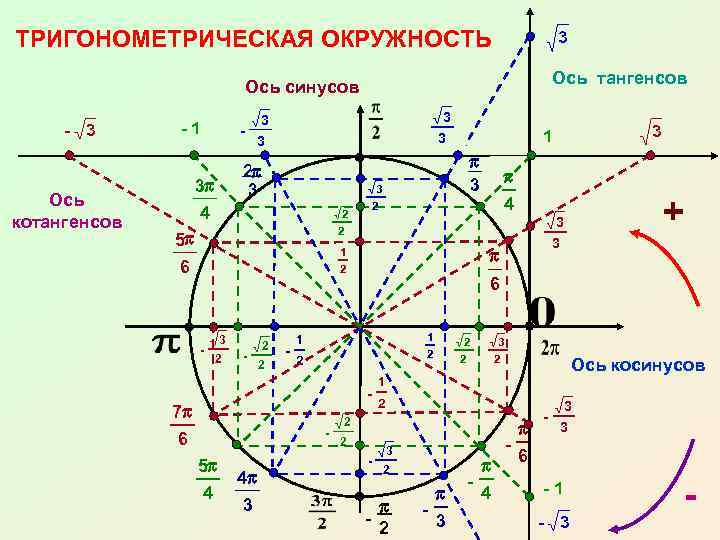
\includegraphics[width=0.7\linewidth]{photo/trigcirc}
		\caption{Тригонометрическая окружность 1}
		\label{pic_trig1}
	\end{subfigure}
	\begin{subfigure}{.5\linewidth}
		\centering
		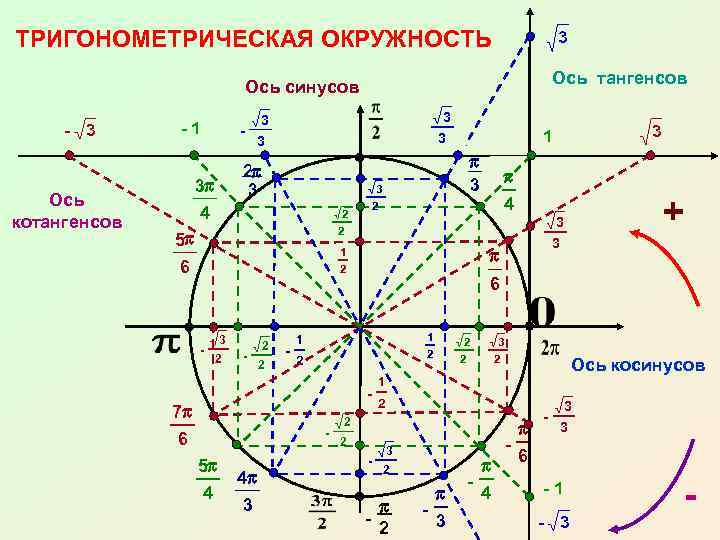
\includegraphics[width=0.7\linewidth]{photo/trigcirc}
		\caption{Тригонометрическая окружность 2}
		\label{pic_trig2}
	\end{subfigure}
\caption{nhb}
\end{figure}

\newpage

\section{Программирование}

Это --- пример наипростейжей программы на C++:

%\begin{lstlisting}[language=C++]
%#include <iostream>
%
%int main()
%{
%	std::cout << "Hello, World!" << std::endl;
%	return 0;
%}	
%\end{lstlisting}

\lstinputlisting{resources/main.cpp}

\begin{verbatim}
#include <iostream>

int main()
{
	std::cout << "Hello, World!" << std::endl;
	return 0;
}
\end{verbatim}

Здесь, \verb|#include <iostream>| --- Подключение библиотеки, позволяющей выводить сообщения на экран.

\newpage

\begin{enumerate} 
	\item текст
	\begin{enumerate} 
		\item текст
		\begin{enumerate} 
			\item текст
			\item текст
		\end{enumerate}
		\item текст
	\end{enumerate} 
	\item текст
\end{enumerate}
\begin{itemize}
	\item текст
	\item текст
	\begin{itemize}
		\item текст
		\begin{itemize}
			\item текст
			\begin{itemize}
				\item текст
			\end{itemize}
		\end{itemize}
	\end{itemize}
\end{itemize}


\end{document} %конец документа